\section{Modelo de levitador magnético}

La dinámica del imán en el sistema de levitación magnética ECP~\cite{730}, con la bobina superior activada, obedece la segunda ley de Newton,
\begin{equation}
m\ddot{x} = f_{\text{fld}}(u,x) - f_{\text{fr}} - mg .
\label{eq:mec}
\end{equation}
En la ecuación de movimiento~\eqref{eq:mec}, $m$ es la masa del imán, en kilogramos, y $\ddot{x}$ su aceleración, en $\text{cm}/\text{s}^2$. La fuerza electromagnética $f_{\text{fld}}$ que ejerce la bobina depende del voltaje aplicado $u$ y de la posición $x$, y se opone al peso $mg$ del imán. La fuerza de fricción $f_{\text{fr}}$ proviene del contacto del imán con su varilla guía. Todas las fuerzas se expresan en $\text{kg}\cdot\text{cm}/\text{s}^2$, en coherencia con los parámetros de la tabla~\ref{tab:parametros}.

La posición $x$ del imán levitante se mide sobre el eje vertical y crece hacia la bobina superior; con el modelo de fuerza que se adopta más adelante, la distancia entre el imán y esa bobina es $a-x$. Por ello, los valores negativos de $x$ que se emplean en este trabajo corresponden a posiciones más alejadas de la bobina, que requieren un voltaje de equilibrio mayor. La figura~\ref{fig:dispositivo} muestra el esquema del dispositivo y las fuerzas que actúan sobre el imán.

\begin{figure}[ht]
    \centering
    % Esquema del ECP-730 en configuración atractiva (notación de la tesis).
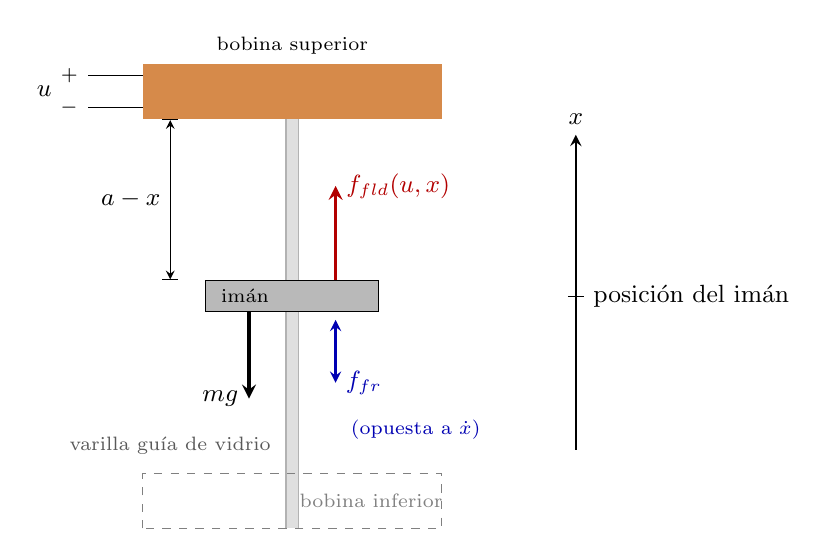
\begin{tikzpicture}[>=stealth, font=\small]
  \definecolor{cobre}{RGB}{214,138,74}
  % varilla guía
  \fill[gray!25] (-0.08,-3.6) rectangle (0.08,2.15);
  \draw[gray!60] (-0.08,-3.6) -- (-0.08,2.15) (0.08,-3.6) -- (0.08,2.15);
  \node[gray!70!black, anchor=east, font=\scriptsize] at (-0.15,-2.55) {varilla guía de vidrio};
  % bobina superior (activa)
  \fill[cobre] (-1.9,1.6) rectangle (1.9,2.3);
  \node[above, font=\scriptsize] at (0,2.3) {bobina superior};
  \draw (-1.9,2.15) -- (-2.6,2.15) node[left, font=\scriptsize] {$+$};
  \draw (-1.9,1.75) -- (-2.6,1.75) node[left, font=\scriptsize] {$-$};
  \node at (-3.15,1.95) {$u$};
  % bobina inferior (inactiva en esta configuración)
  \draw[dashed, gray] (-1.9,-3.6) rectangle (1.9,-2.9);
  \node[gray, font=\scriptsize] at (1.0,-3.25) {bobina inferior};
  % imán levitante
  \fill[gray!55] (-1.1,-0.85) rectangle (1.1,-0.45);
  \draw (-1.1,-0.85) rectangle (1.1,-0.45);
  \node[font=\scriptsize] at (-0.6,-0.65) {imán};
  % fuerzas
  \draw[->, very thick, red!70!black] (0.55,-0.45) -- (0.55,0.75) node[right] {$f_{\text{fld}}(u,x)$};
  \draw[->, very thick] (-0.55,-0.85) -- (-0.55,-1.95) node[left] {$mg$};
  \draw[<->, thick, blue!70!black] (0.55,-0.95) -- (0.55,-1.75) node[right] {$f_{\text{fr}}$};
  \node[blue!70!black, font=\scriptsize, anchor=north west] at (0.62,-2.1) {(opuesta a $\dot x$)};
  % distancia a la bobina
  \draw[|<->|, thin] (-1.55,-0.45) -- (-1.55,1.6) node[midway, left] {$a-x$};
  % eje x
  \draw[->, thick] (3.6,-2.6) -- (3.6,1.4) node[above] {$x$};
  \draw (3.5,-0.65) -- (3.7,-0.65) node[right] {posición del imán};
\end{tikzpicture}

    \caption[Esquema del ECP-730 en configuración atractiva]{Esquema del sistema de levitación ECP-730 en configuración atractiva. La bobina superior atrae al imán, que se desliza sobre una varilla guía; el contacto entre ambos produce la fricción $f_{\text{fr}}$. La bobina inferior solo se emplea en la configuración repulsiva.}
    \label{fig:dispositivo}
\end{figure}

\section{\texorpdfstring{Formas de $f_{\text{fld}}$}{Formas de fld}}

La literatura documenta varias formas no lineales para la fuerza electromagnética, que dependen de cómo varía la inductancia de la bobina con la posición del objeto levitante. De acuerdo con Al-Muthair et al.~\cite{al}, la fuerza sobre una bola ferromagnética levitada se aproxima por
\begin{equation}
f_{\text{fld}} = C\left(\dfrac{i}{x}\right)^2 .
\label{eq:fld_al}
\end{equation}
En la aproximación de Al-Muthair~\eqref{eq:fld_al}, la fuerza crece con el cuadrado de la intensidad de corriente $i$ y decrece con el cuadrado de la posición $x$ de la bola. La constante $C$ de la fuerza magnética reúne las propiedades del electroimán.

Charara et al.~\cite{charara} calculan la fuerza electromagnética dentro de un cojinete magnético como
\begin{equation}
f_{\text{fld}} = K\,\frac{\operatorname{sign}(i)\,i^{2}}{e^{2}},
\qquad
K = 0{,}25 \cos\!\left(\frac{\pi}{8}\right)\!\mu\, n^{2} S .
\label{eq:fld_charara}
\end{equation}
En el modelo del cojinete~\eqref{eq:fld_charara}, la fuerza conserva el signo de la corriente $i$ y decrece con el cuadrado del entrehierro $e$. La constante $K$ depende del área $S$ de la cara del polo, de la permeabilidad magnética del vacío $\mu$ y del número $n$ de vueltas del embobinado.

El Hajjaji et al.~\cite{el} determinaron experimentalmente que la fuerza electromagnética sobre una esfera metálica tiene la forma
\begin{equation}
f_{\text{fld}} = \dfrac{i^{2}}{b_0 + b_1x + b_2x^3 + b_3x^4} .
\label{eq:fld_hajjaji}
\end{equation}
Los coeficientes del ajuste experimental~\eqref{eq:fld_hajjaji} son $b_0=0{,}0304$, $b_1=0{,}7159$, $b_2=-0{,}9165$ y $b_3=1{,}1994$.

Zhao et al.~\cite{zhao} calculan la fuerza del electroimán que hace levitar una bola metálica como
\begin{equation}
f_{\text{fld}} = \frac{L_0 x_0 i^2}{2x^2} .
\label{eq:fld_zhao}
\end{equation}
La fuerza del modelo de Zhao~\eqref{eq:fld_zhao} crece con el cuadrado de la corriente $i$ del embobinado y decrece con el cuadrado de la posición $x$ de la bola. Su escala la fija la inductancia $L_0$ del sistema en el punto de equilibrio $x_0$.

Zhang et al.~\cite{feifei} determinan, para un sistema similar, la fuerza electromagnética
\begin{equation}
f_{\text{fld}} = \frac{K i^2}{(H - x)^2} .
\label{eq:fld_zhang}
\end{equation}
La fuerza del modelo de Zhang~\eqref{eq:fld_zhang} también crece con el cuadrado de la intensidad de la corriente $i$, y su denominador depende de la posición $x$ del objeto. Las constantes $K$ y $H$ son parámetros del sistema.

Cada uno de estos modelos está condicionado por la configuración del sistema y por la metodología, analítica o experimental, con que se obtuvo. Por ello, en este trabajo se adopta el modelo del levitador ECP-730 que da el fabricante en su hoja de especificaciones~\cite{parks}, validado experimentalmente por Alcántara et al.~\cite{alcantara},
\begin{equation}
f_{\text{fld}} = \frac{u}{b(a-x)^4} .
\label{eq:fld}
\end{equation}
La fuerza del fabricante~\eqref{eq:fld} es proporcional al voltaje $u$ aplicado en las terminales del embobinado del electroimán y decrece con la cuarta potencia de la distancia $a-x$ entre el imán, en la posición $x$, y la bobina. Los parámetros $a$ y $b$ son propios del dispositivo y se reúnen en la tabla~\ref{tab:parametros}.

\section{Zona muerta dinámica no centrada en el origen}
Pérez-Gómez~\cite{perez} sostiene que la zona muerta dura describe con mayor precisión el fenómeno observado en motores eléctricos, en los que esta no linealidad se centra en $u_e(t) = 0$, el único voltaje de equilibrio de los sistemas de control de posición angular.

En los sistemas de levitación magnética, en cambio, cada posición tiene su propio voltaje de equilibrio $u_e$, y la zona muerta se centra en él,
\begin{equation}
v(t) = D\big(u(t)\big) =
\begin{cases}
m_r \big(u(t) - u_e - b_r\big) - h_r, & u(t) - u_e \ge b_r, \\[6pt]
0, & b_l < u(t) - u_e < b_r, \\[6pt]
m_l \big(u(t) - u_e - b_l\big) - h_l, & u(t) - u_e \le b_l.
\end{cases}
\label{eq:zm}
\end{equation}
La zona muerta~\eqref{eq:zm} transforma el voltaje comandado $u$ en la salida $v$ del actuador. Mientras la desviación $u-u_e$ permanece entre los umbrales $b_l$ y $b_r$, la salida es nula. Fuera de esa banda, la salida crece con las pendientes $m_r$ y $m_l$ y se desplaza por los saltos $h_r$ y $h_l$. Estos seis parámetros son desconocidos, pero sus signos se conocen: $m_r > 0$, $m_l > 0$, $b_r > 0$, $b_l < 0$, $h_r < 0$ y $h_l > 0$.

Como estos parámetros no se conocen para el ECP-730, en las simulaciones se emplea una implementación simplificada con la misma asimetría de signos. Mientras el levitante está en movimiento, el actuador no responde a cambios del voltaje comandado comprendidos entre $-0{,}02$ y $+0{,}025$~V respecto al último voltaje aplicado, que se mantiene; los cambios mayores se transmiten sin modificación. Cuando el levitante está atascado, el voltaje comandado se aplica directamente. La identificación de los parámetros de $D(u)$ se propone como trabajo futuro.

\begin{figure}[ht]
    \centering
    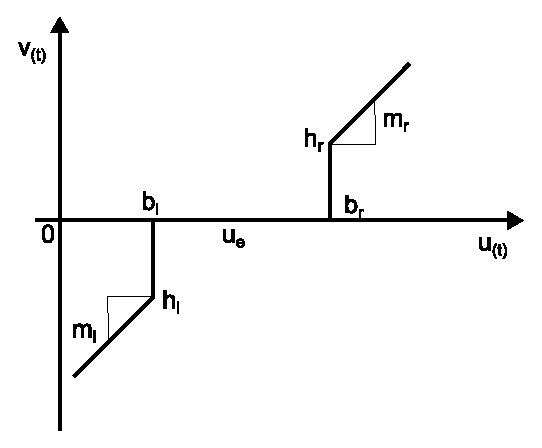
\includegraphics[width=0.45\textwidth]{images/chapter_1/zm_levitador.eps}
    \caption[Zona muerta centrada en el voltaje de equilibrio]{Zona muerta $v=D(u)$ centrada en el voltaje de equilibrio $u_e$, con pendientes $m_l$, $m_r$, umbrales $b_l$, $b_r$ y saltos $h_l$, $h_r$.}
    \label{fig:zm}
\end{figure}

La figura~\ref{fig:zm} muestra la forma de $D(u)$: mientras el voltaje comandado se mantenga dentro de la banda $(u_e+b_l,\,u_e+b_r)$, la salida $v$ del actuador es nula.

\section{Efecto atascamiento-deslizamiento}
El atascamiento-deslizamiento es característico de los sistemas con fricción en los que el movimiento alterna intervalos de atascamiento, sin movimiento, con deslizamientos repentinos. Los modelos de fricción documentados buscan reproducir este comportamiento~\cite{armstrong,olsson,berman}. En este trabajo se emplea un modelo de fricción compuesto. Con velocidad nula, el sistema está en régimen de fricción estática; cuando la fuerza externa lo pone en movimiento, la fricción disminuye de golpe y el sistema pasa al régimen de fricción dinámica. La alternancia entre ambos regímenes es el efecto atascamiento-deslizamiento. La fuerza de fricción es
\begin{equation}
f_{\text{fr}} =
\begin{cases}
m\,c_1\,v,
& v \neq 0, \\[6pt]
\min\!\left(|F_e|,\,F_s\right)\,\operatorname{sign}(F_e),
& v = 0 .
\end{cases}
\label{eq:friccion}
\end{equation}
En el régimen de deslizamiento, la fricción~\eqref{eq:friccion} es viscosa y proporcional a la velocidad relativa $v$ del imán, con el coeficiente $c_1$ de fricción viscosa por unidad de masa. En reposo, la fricción equilibra la fuerza externa $F_e(t)$ que actúa sobre el imán hasta un valor máximo $F_s$, la fricción estática máxima.

Cuando las transiciones entre ambos regímenes se repiten de manera regular, dan lugar a un ciclo límite.



La figura~\ref{lazo_de_control_con_zm} muestra el lazo de control completo, con la zona muerta entre el controlador y la planta.
\begin{figure}[ht]
    \centering
       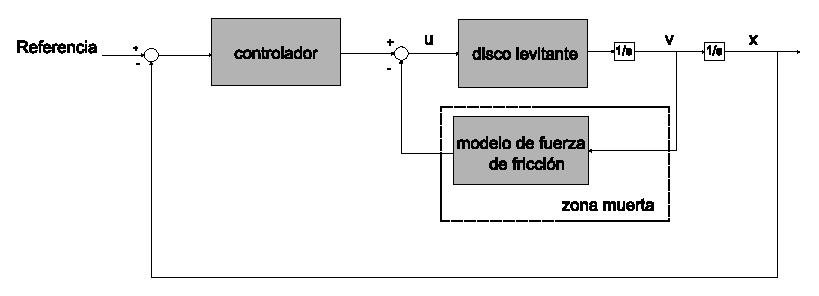
\includegraphics[width=0.6\textwidth]{images/chapter_1/lazo_de_control_con_zm.eps}
    \caption{Lazo de control con zona muerta}
    \label{lazo_de_control_con_zm}
\end{figure}

\section{Soluciones numéricas}
El atascamiento-deslizamiento es difícil de simular en sistemas de control con componentes mecánicos, porque la fuerza de fricción es discontinua en la velocidad cero. Alrededor de ese punto la dificultad es más numérica que física, y existe una amplia variedad de estrategias para modelarla e implementarla, conocidas como modelos dinámicos de fricción~\cite{haessig}.

El método de Karnopp~\cite{karnopp} introduce una banda de velocidad $|v| \le DV$ que se trata como velocidad cero, y con ella decide si el sistema está atascado o deslizando. Por su fácil implementación se emplea en aplicaciones prácticas de diseño de actuadores~\cite{liu,ravanbod,ravanbod1,bicakci,romano}, y por ello se utiliza también en las simulaciones de este trabajo.

\section{Modelo linealizado del sistema de levitación magnética}
Los parámetros del modelo no lineal ($a$, $b$, $c_1$, $m$, $g$) fueron identificados experimentalmente por Hernández Alcántara~\cite{diana_tesis} para el dispositivo ECP-730 en configuración repulsiva (estable en lazo abierto), mediante ensayos de estado estacionario y respuesta dinámica en lazo abierto. En el presente trabajo se adoptan esos mismos parámetros y se aplican a la configuración atractiva (inestable en lazo abierto), en la que la bobina superior atrae al imán levitante. La estructura funcional del modelo es idéntica en ambas configuraciones; en la atractiva, la fuerza magnética crece al disminuir la brecha entre el imán y la bobina, lo que hace que los puntos de equilibrio sean inestables. El modelo linealizado en espacio de estados para la configuración inestable es
\begin{equation}
\begin{aligned}
\dot{x}
&=
\begin{bmatrix}
0 & 1 \\[6pt]
\dfrac{4g}{(a-x_1^{\ast})} & -c_1
\end{bmatrix}x
+
\begin{bmatrix}
0 \\[6pt]
\dfrac{1}{mb\,(a-x_1^{\ast})^4}
\end{bmatrix}u,
\\[10pt]
y &= \begin{bmatrix} 1 & 0 \end{bmatrix} x .
\end{aligned}
\label{eq:lineal}
\end{equation}
En el modelo linealizado~\eqref{eq:lineal}, el vector de estado $x$ reúne la posición $x_1$ y la velocidad $x_2$ del imán, y la salida $y$ es la posición. La linealización se hace alrededor de la posición de equilibrio $x_1^{\ast}$. El coeficiente $c_1$ de fricción viscosa por unidad de masa aparece en la matriz de estado como un amortiguamiento.

Su ecuación característica es
\begin{equation}
\lambda^2 + c_1\lambda - \dfrac{4g}{(a-x_1^{\ast})} = 0 .
\label{eq:caracteristica}
\end{equation}
Como $a - x_1^{\ast} > 0$ para toda posición alcanzable, el término independiente de la ecuación característica~\eqref{eq:caracteristica} es negativo y la ecuación tiene siempre una raíz real positiva: todos los puntos de equilibrio de la configuración atractiva son inestables. En $x_1^{\ast}=-4$~cm las raíces son $\lambda_1 = -23{,}5057$ y $\lambda_2 = 14{,}9427$.

Las matrices de controlabilidad y de observabilidad del modelo linealizado son
\begin{equation}
\mathcal{C}
=
\begin{bmatrix}
0 & \beta\\[6pt]
\beta & -c_1 \beta
\end{bmatrix} ,
\qquad
\mathcal{O}
=
\begin{bmatrix}
1 & 0\\[6pt]
0 & 1
\end{bmatrix} .
\label{eq:ctrb_obsv}
\end{equation}
La constante $\beta = 1/[m\,b\,(a-x_1^{\ast})^4]$ es la ganancia con la que el voltaje entra en la aceleración del imán. Las dos matrices~\eqref{eq:ctrb_obsv} tienen rango completo, de modo que el sistema es controlable y observable: con la entrada de la planta se puede llevar el estado a cualquier punto del espacio de estados, y a partir de la salida se puede determinar en qué punto se encuentra.
Los valores de $c_1$, $b$, $a$, $m$ y $g$ que se emplearon en los cálculos fueron identificados experimentalmente por Hernández Alcántara~\cite{diana_tesis}; se reúnen en la tabla~\ref{tab:parametros} junto con los parámetros del modelo de fricción y el intervalo de la señal de control. Las fuerzas se expresan en $\text{kg}\cdot\text{cm}/\text{s}^2$, unidades en las que el peso del imán es $mg = 138{,}3$. En la tesis de Hernández Alcántara~\cite{diana_tesis}, $c_1$ se reporta en $\text{kg}^{-1}$; dado que multiplica a la velocidad en la ecuación de aceleración, sus unidades consistentes son $\text{s}^{-1}$.

\begin{table}[ht]
\centering
\caption{Parámetros del modelo}
\label{tab:parametros}
\begin{tabular}{|c|c|l|}
\hline
$a$ & $7{,}17184\;[\text{cm}]$ & parámetro de la fuerza electromagnética \\ \hline
$b$ & $1{,}6163 \times 10^{-6}\;[\text{V}/(\text{N}\cdot\text{cm}^4)]$ & parámetro de la fuerza electromagnética \\ \hline
$c_1$ & $8{,}563\;[\text{s}^{-1}]$ & fricción viscosa por unidad de masa \\ \hline
$m$ & $0{,}141\;[\text{kg}]$ & masa del imán levitante \\ \hline
$g$ & $981\;[\text{cm}/\text{s}^2]$ & aceleración de la gravedad \\ \hline
$F_s$ & $20\;[\text{kg}\cdot\text{cm}/\text{s}^2]$ ($0{,}2$~N) & fricción estática máxima (Karnopp) \\ \hline
$DV$ & $0{,}02\;[\text{cm}/\text{s}]$ & banda de velocidad nula (Karnopp) \\ \hline
$u$ & $[0;\ 3{,}5]\;[\text{V}]$ & intervalo de la señal de control \\ \hline
$[b_l,\,b_r]$ & $[-0{,}02;\ +0{,}025]\;[\text{V}]$ & banda de la zona muerta simulada \\ \hline
\end{tabular}
\end{table}


% Generado a partir de calculus/Final_Bien/evidencia_P8.m (simulador corregido).
\subsection{Sistema no lineal en lazo abierto en los puntos de equilibrio}

Para caracterizar la inestabilidad de la configuración atractiva, se simuló el modelo no lineal sin fricción estática ni zona muerta, aplicando el voltaje de equilibrio $u=u_e(x_1^*)$ y desplazando la posición inicial $0{,}01$~cm respecto al equilibrio, en $x_1^*=-4$, $-3$ y $-2$~cm. La figura~\ref{fig:p8_lazo_abierto} muestra que la desviación crece exponencialmente y alcanza 1~cm en $0{,}33$, $0{,}32$ y $0{,}30$~s, respectivamente; el modelo linealizado reproduce el crecimiento con un tiempo de duplicación $\ln 2/\lambda_2$ de $46$, $44$ y $41$~ms. Cuanto más cerca de la bobina se encuentra el equilibrio, más rápido es el polo inestable.

\begin{figure}[ht]
    \centering
    % Estilo común de las figuras de evidencia P8 (pgfplots).
\pgfplotsset{
  pocho/.style={
    width=0.92\textwidth, height=5.2cm,
    grid=major, grid style={gray!25},
    tick label style={font=\small}, label style={font=\small}, legend style={font=\small},
    /pgf/number format/use comma,
    scaled ticks=false,
    y tick label style={/pgf/number format/fixed},
    table/col sep=comma, unbounded coords=jump,
    every axis plot/.append style={line join=round},
  },
}
\definecolor{tray}{RGB}{31,94,166}
\definecolor{refc}{RGB}{40,40,40}
\definecolor{ctl2}{RGB}{196,96,40}
\definecolor{ver}{RGB}{46,133,64}

\begin{tikzpicture}
\begin{semilogyaxis}[pocho, height=6cm, xmin=0, xmax=0.36, ymin=0.01, ymax=1,
    xlabel={tiempo [\si{s}]}, ylabel={$|x_1(t)-x_1^*|$ [\si{cm}]},
    x tick label style={/pgf/number format/fixed},
    legend style={at={(0.02,0.98)}, anchor=north west}, legend cell align=left]
  \addplot[tray, line width=1pt]  table[x=t, y=nl_m4] {images/p8_results/tikz/lazo_abierto.csv}; \addlegendentry{$x_1^*=-4$ cm}
  \addplot[ctl2, line width=1pt]  table[x=t, y=nl_m3] {images/p8_results/tikz/lazo_abierto.csv}; \addlegendentry{$x_1^*=-3$ cm}
  \addplot[ver, line width=1pt]   table[x=t, y=nl_m2] {images/p8_results/tikz/lazo_abierto.csv}; \addlegendentry{$x_1^*=-2$ cm}
  \addplot[tray, densely dashed]  table[x=t, y=lin_m4] {images/p8_results/tikz/lazo_abierto.csv}; \addlegendentry{modelo lineal}
  \addplot[ctl2, densely dashed, forget plot] table[x=t, y=lin_m3] {images/p8_results/tikz/lazo_abierto.csv};
  \addplot[ver, densely dashed, forget plot]  table[x=t, y=lin_m2] {images/p8_results/tikz/lazo_abierto.csv};
\end{semilogyaxis}
\end{tikzpicture}

    \caption[Lazo abierto en los puntos de equilibrio]{Desviación respecto al equilibrio en lazo abierto, con $u=u_e$ y una perturbación inicial de $0{,}01$~cm. Líneas continuas: modelo no lineal; discontinuas: modelo linealizado.}
    \label{fig:p8_lazo_abierto}
\end{figure}

El retrato de fase alrededor de $x_1^*=-4$~cm (figura~\ref{fig:p8_retrato}) confirma que el equilibrio es un punto silla: las trayectorias se alejan a lo largo de la variedad inestable, salvo las que parten exactamente sobre la variedad estable. Al incorporar la fricción estática de Karnopp cambia la situación en reposo: si el levitante está detenido y $u=u_e$, la fuerza neta $u/[b(a-x)^4]-mg$ no supera $F_s$ mientras la posición se encuentre entre $-4{,}44$ y $-3{,}63$~cm, de modo que el imán permanece atascado en cualquier punto de esa banda. Para $x_1^*=-3$ y $-2$~cm las bandas correspondientes son $[-3{,}41;\,-2{,}66]$ y $[-2{,}37;\,-1{,}70]$~cm. La fricción estática enmascara así la inestabilidad del equilibrio mientras el levitante no se mueva.

\begin{figure}[ht]
    \centering
    % Estilo común de las figuras de evidencia P8 (pgfplots).
\pgfplotsset{
  pocho/.style={
    width=0.92\textwidth, height=5.2cm,
    grid=major, grid style={gray!25},
    tick label style={font=\small}, label style={font=\small}, legend style={font=\small},
    /pgf/number format/use comma,
    scaled ticks=false,
    y tick label style={/pgf/number format/fixed},
    table/col sep=comma, unbounded coords=jump,
    every axis plot/.append style={line join=round},
  },
}
\definecolor{tray}{RGB}{31,94,166}
\definecolor{refc}{RGB}{40,40,40}
\definecolor{ctl2}{RGB}{196,96,40}
\definecolor{ver}{RGB}{46,133,64}

\begin{tikzpicture}
\begin{axis}[pocho, width=0.8\textwidth, height=7.5cm, xmin=-4.5, xmax=-3.5, ymin=-10, ymax=10,
    xlabel={posición $x_1$ [\si{cm}]}, ylabel={velocidad $x_2$ [\si{cm/s}]},
    legend style={at={(0.98,0.02)}, anchor=south east, fill=white}, legend cell align=left]
  \addplot[gray!60, quiver={u=\thisrow{dx}, v=\thisrow{dv}, every arrow/.append style={-stealth}}, forget plot]
    table[x=x, y=v] {images/p8_results/tikz/campo.csv};
  \addplot[tray, line width=0.9pt] table[x=x, y=v] {images/p8_results/tikz/trayectorias.csv}; \addlegendentry{trayectorias}
  \addplot[ctl2, line width=1.4pt] table[x=x, y=v] {images/p8_results/tikz/variedad_inestable.csv}; \addlegendentry{variedad inestable}
  \addplot[ver, line width=3pt, opacity=0.6] coordinates {(-4.4448,0) (-3.6291,0)}; \addlegendentry{banda de atascamiento ($u=u_e$)}
  \addplot[only marks, mark=*, mark size=2pt, refc] coordinates {(-4,0)}; \addlegendentry{equilibrio $x_1^*=-4$ cm}
\end{axis}
\end{tikzpicture}

    \caption[Retrato de fase en lazo abierto]{Retrato de fase del modelo no lineal sin fricción estática alrededor de $x_1^*=-4$~cm, con $u=u_e$. La banda verde indica las posiciones en las que, con el levitante en reposo, la fricción estática lo mantiene atascado.}
    \label{fig:p8_retrato}
\end{figure}

\FloatBarrier


\subsection{Control con doble acción integral}
\label{sec:pii}
El controlador se ajustó sobre el modelo linealizado en $x_1^*=-4$~cm, de forma interactiva en los editores de Bode y del lugar de las raíces del \emph{Control System Designer} de MATLAB. La motivación de la doble acción integral fue proporcionar alta ganancia a baja frecuencia, con la expectativa de acelerar la salida de la zona muerta y reducir el tiempo de atascamiento respecto a un PI; esa expectativa se evalúa en el capítulo~\ref{chap:resultados}. El controlador resultante es
\begin{equation}
C(s)=\frac{152{,}43\,(s+4{,}875)(s+1{,}861)(s+17{,}31)}
{s^{2}(s+301{,}1)} .
\label{eq:pii}
\end{equation}

\begin{figure}[ht]
    \centering
    % Estilo común de las figuras de diseño del PII (pgfplots).
% Generado por diseno_PII_tikz.m
\def\PIIwg{9.6320}
\def\PIImgwg{17.0713}
\def\PIIwp{129.2942}
\def\PIIphwp{-120.1396}
\def\PIIgmdb{-17.1}
\def\PIIpm{59.9}
\def\PIIos{16.9}
\def\PIIts{0.284}
\def\PIItp{0.0238}
\def\PIIyp{1.1688}
\def\PIIflechaA{(-7.6265,1.7150) -- (-7.5765,1.4566)}
\def\PIIflechaC{(-7.5765,-1.4566) -- (-7.6265,-1.7150)}
\def\PIIflechaB{(-2.6114,-3.2049) -- (-2.5176,-3.1809)}
\def\PIIflechaD{(-2.5176,3.1809) -- (-2.6114,3.2049)}

\pgfplotsset{
  diseno/.style={
    grid=major, grid style={gray!25},
    tick label style={font=\small}, label style={font=\small}, legend style={font=\small},
    /pgf/number format/use comma,
    table/col sep=comma,
    every axis plot/.append style={line join=round},
  },
}
\definecolor{tray}{RGB}{31,94,166}
\definecolor{marg}{RGB}{196,96,40}
\definecolor{refc}{RGB}{40,40,40}

\begin{tikzpicture}
\begin{axis}[diseno, name=mag, width=0.85\textwidth, height=5.2cm, xmode=log,
             xmin=1e-2, xmax=1e4, ymin=-100, ymax=110, ytick={-100,-50,0,50,100},
             xticklabels={}, ylabel={magnitud [\si{dB}]}]
  \addplot[refc!50, densely dashed] coordinates {(1e-2,0) (1e4,0)};
  \addplot[tray, line width=1pt] table[x=w, y=mag_db] {images/pii_design/tikz/bode.csv};
  \draw[marg, line width=0.8pt] (axis cs:\PIIwg,0) -- (axis cs:\PIIwg,\PIImgwg);
  \addplot[marg, only marks, mark=*, mark size=1.8pt] coordinates {(\PIIwg,\PIImgwg)};
  \node[font=\small, anchor=north east, align=left, fill=white, inner sep=2pt]
    at (axis cs:8e3,104) {MG $=\num{\PIIgmdb}$~\si{dB} en $\omega=\num[round-mode=places,round-precision=2]{\PIIwg}$~\si{rad/s}};
\end{axis}
\begin{axis}[diseno, at={(mag.south west)}, anchor=north west, yshift=-0.35cm,
             width=0.85\textwidth, height=5.2cm, xmode=log,
             xmin=1e-2, xmax=1e4, ymin=-375, ymax=-90, ytick={-360,-315,-270,-225,-180,-135},
             xlabel={frecuencia [\si{rad/s}]}, ylabel={fase [\si{\degree}]}]
  \addplot[refc!50, densely dashed] coordinates {(1e-2,-180) (1e4,-180)};
  \addplot[tray, line width=1pt] table[x=w, y=fase] {images/pii_design/tikz/bode.csv};
  \draw[marg, line width=0.8pt] (axis cs:\PIIwp,-180) -- (axis cs:\PIIwp,\PIIphwp);
  \addplot[marg, only marks, mark=*, mark size=1.8pt] coordinates {(\PIIwp,\PIIphwp)};
  \node[font=\small, anchor=south east, align=left, fill=white, inner sep=2pt]
    at (axis cs:8e3,-370) {MF $=\num{\PIIpm}\si{\degree}$ en $\omega=\num[round-mode=places,round-precision=1]{\PIIwp}$~\si{rad/s}};
\end{axis}
\end{tikzpicture}

    \caption[Diagrama de Bode]{Diagrama de Bode del lazo abierto $L(s)=C(s)G(s)$ en $x_1^*=-4$~cm. Se indican el margen de ganancia (inferior, por el polo inestable de la planta) y el margen de fase.}
    \label{bode_fase}
\end{figure}

\begin{figure}[ht]
    \centering
    % Estilo común de las figuras de diseño del PII (pgfplots).
% Generado por diseno_PII_tikz.m
\def\PIIwg{9.6320}
\def\PIImgwg{17.0713}
\def\PIIwp{129.2942}
\def\PIIphwp{-120.1396}
\def\PIIgmdb{-17.1}
\def\PIIpm{59.9}
\def\PIIos{16.9}
\def\PIIts{0.284}
\def\PIItp{0.0238}
\def\PIIyp{1.1688}
\def\PIIflechaA{(-7.6265,1.7150) -- (-7.5765,1.4566)}
\def\PIIflechaC{(-7.5765,-1.4566) -- (-7.6265,-1.7150)}
\def\PIIflechaB{(-2.6114,-3.2049) -- (-2.5176,-3.1809)}
\def\PIIflechaD{(-2.5176,3.1809) -- (-2.6114,3.2049)}

\pgfplotsset{
  diseno/.style={
    grid=major, grid style={gray!25},
    tick label style={font=\small}, label style={font=\small}, legend style={font=\small},
    /pgf/number format/use comma,
    table/col sep=comma,
    every axis plot/.append style={line join=round},
  },
}
\definecolor{tray}{RGB}{31,94,166}
\definecolor{marg}{RGB}{196,96,40}
\definecolor{refc}{RGB}{40,40,40}

\begin{tikzpicture}
\begin{axis}[diseno, width=0.8\textwidth, height=0.62\textwidth,
             xmin=-10, xmax=2, ymin=-7, ymax=7, axis equal image,
             xlabel={$\operatorname{Re}\{L(j\omega)\}$}, ylabel={$\operatorname{Im}\{L(j\omega)\}$},
             legend pos=north west, legend cell align=left]
  \addplot[refc!40, thin, forget plot] coordinates {(-10,0) (2,0)};
  \addplot[refc!40, thin, forget plot] coordinates {(0,-7) (0,7)};
  \addplot[refc!55, densely dashed, domain=0:360, samples=120, forget plot] ({cos(x)},{sin(x)});
  \addplot[tray, line width=1pt]
    table[x=re, y=im] {images/pii_design/tikz/nyquist_pos.csv};
  \addlegendentry{$\omega>0$}
  \addplot[tray!55, line width=0.8pt, densely dashed]
    table[x=re, y=im] {images/pii_design/tikz/nyquist_neg.csv};
  \addlegendentry{$\omega<0$}
  \addplot[red!75!black, only marks, mark=+, mark size=4pt, line width=1.2pt] coordinates {(-1,0)};
  \addlegendentry{$-1$}
  \draw[tray, -stealth, line width=1pt] \PIIflechaA;
  \draw[tray, -stealth, line width=1pt] \PIIflechaB;
  \draw[tray!55, -stealth, line width=0.8pt] \PIIflechaC;
  \draw[tray!55, -stealth, line width=0.8pt] \PIIflechaD;
  \draw[marg, thin] (axis cs:-7.14,0) -- (axis cs:-8.5,-1.2);
  \node[font=\small, anchor=north, fill=white, inner sep=1.5pt] at (axis cs:-8.5,-1.2) {$-1/\mathrm{MG}$};
  \addplot[marg, only marks, mark=*, mark size=1.6pt, forget plot] coordinates {(-7.14,0)};
\end{axis}
\end{tikzpicture}

    \caption[Diagrama de Nyquist]{Diagrama de Nyquist de $L(s)$. Con un polo de lazo abierto en el semiplano derecho ($P=1$), la estabilidad en lazo cerrado exige un rodeo antihorario al punto $-1$.}
    \label{nyquist}
\end{figure}

\begin{figure}[ht]
    \centering
    % Estilo común de las figuras de diseño del PII (pgfplots).
% Generado por diseno_PII_tikz.m
\def\PIIwg{9.6320}
\def\PIImgwg{17.0713}
\def\PIIwp{129.2942}
\def\PIIphwp{-120.1396}
\def\PIIgmdb{-17.1}
\def\PIIpm{59.9}
\def\PIIos{16.9}
\def\PIIts{0.284}
\def\PIItp{0.0238}
\def\PIIyp{1.1688}
\def\PIIflechaA{(-7.6265,1.7150) -- (-7.5765,1.4566)}
\def\PIIflechaC{(-7.5765,-1.4566) -- (-7.6265,-1.7150)}
\def\PIIflechaB{(-2.6114,-3.2049) -- (-2.5176,-3.1809)}
\def\PIIflechaD{(-2.5176,3.1809) -- (-2.6114,3.2049)}

\pgfplotsset{
  diseno/.style={
    grid=major, grid style={gray!25},
    tick label style={font=\small}, label style={font=\small}, legend style={font=\small},
    /pgf/number format/use comma,
    table/col sep=comma,
    every axis plot/.append style={line join=round},
  },
}
\definecolor{tray}{RGB}{31,94,166}
\definecolor{marg}{RGB}{196,96,40}
\definecolor{refc}{RGB}{40,40,40}

\begin{tikzpicture}
\begin{axis}[diseno, width=0.85\textwidth, height=6cm, xmin=0, xmax=0.6, ymin=0, ymax=1.32,
             xlabel={tiempo [\si{s}]}, ylabel={amplitud},
             xtick={0,0.1,...,0.6}, x tick label style={/pgf/number format/fixed}]
  \addplot[refc!55, densely dashed] coordinates {(0,1) (0.6,1)};
  \addplot[refc!30, densely dotted, forget plot] coordinates {(0,0.98) (0.6,0.98)};
  \addplot[refc!30, densely dotted, forget plot] coordinates {(0,1.02) (0.6,1.02)};
  \addplot[tray, line width=1pt] table[x=t, y=y] {images/pii_design/tikz/escalon.csv};
  \addplot[marg, only marks, mark=*, mark size=1.8pt] coordinates {(\PIItp,\PIIyp)};
  \node[font=\small, anchor=south west, inner sep=2pt] at (axis cs:\PIItp,\PIIyp)
    {sobrepaso \SI{\PIIos}{\percent}};
  \draw[marg, densely dashed] (axis cs:\PIIts,0) -- (axis cs:\PIIts,0.98);
  \node[font=\small, anchor=south west, fill=white, inner sep=2pt] at (axis cs:\PIIts,0.08)
    {$t_s=\num{\PIIts}$~\si{s} (\SI{2}{\percent})};
\end{axis}
\end{tikzpicture}

    \caption[Respuesta al escalón]{Respuesta al escalón unitario del lazo cerrado linealizado.}
    \label{step_response}
\end{figure}

La estructura del controlador PII~\eqref{eq:pii} tiene tres partes. El doble integrador hace al lazo de tipo dos, lo que anula el error estacionario ante escalones y rampas. Los ceros en $-1{,}861$ y $-4{,}875$~rad/s compensan el atraso de fase de los dos integradores por debajo de la frecuencia de cruce. El par cero-polo en $-17{,}31$ y $-301{,}1$~rad/s actúa como red de adelanto, con su máximo aporte de fase cerca de $72$~rad/s. Con esta estructura, el lazo tiene un margen de fase de $59{,}9^\circ$ en $129{,}3$~rad/s (figura~\ref{bode_fase}). Como la planta tiene un polo inestable, el margen de ganancia es inferior: el lazo sigue siendo estable si la ganancia aumenta, pero se inestabiliza si disminuye por debajo de $0{,}14$ veces su valor nominal ($-17{,}1$~dB en $9{,}63$~rad/s). El diagrama de Nyquist (figura~\ref{nyquist}) rodea una vez el punto $-1$ en sentido antihorario, como exige el criterio con un polo inestable en lazo abierto. En lazo cerrado lineal, la respuesta al escalón (figura~\ref{step_response}) tiene un sobrepaso de $16{,}9$\,\% y un tiempo de establecimiento de $0{,}284$~s.    

\FloatBarrier
\newpage

% Generado a partir de calculus/Final_Bien/evidencia_P8.m (simulador corregido).
\subsection{Controlador con atascamiento-deslizamiento sobre el modelo lineal}

Para separar el efecto de las no linealidades no suaves del de la no linealidad de la fuerza electromagnética, el PII se probó sobre el modelo linealizado en $x_1^*=-2{,}5$~cm al que se añadieron la zona muerta y la fricción de Karnopp, con la misma prueba que se emplea en el capítulo~\ref{chap:resultados} para la regulación del modelo no lineal ($-2\to-3$~cm, $u\in[0;\,3{,}5]$~V). La figura~\ref{fig:p8_lineal_ad} compara ambos resultados. El comportamiento es prácticamente el mismo: sobrepaso de $24{,}4$\,\% frente a $23{,}6$\,\%, entrada en la banda de $\pm5$\,\% en $0{,}41$ frente a $0{,}40$~s y un ciclo límite de $0{,}028$ frente a $0{,}033$~cm pico a pico. La única diferencia apreciable es el voltaje de equilibrio final ($2{,}36$~V en el modelo lineal frente a $2{,}39$~V), consecuencia del error de linealización a $0{,}5$~cm del punto de operación. Esto indica que el ciclo límite se debe a la zona muerta y a la fricción estática, y no a la no linealidad de la fuerza electromagnética.

\begin{figure}[ht]
    \centering
    % Estilo común de las figuras de evidencia P8 (pgfplots).
\pgfplotsset{
  pocho/.style={
    width=0.92\textwidth, height=5.2cm,
    grid=major, grid style={gray!25},
    tick label style={font=\small}, label style={font=\small}, legend style={font=\small},
    /pgf/number format/use comma,
    scaled ticks=false,
    y tick label style={/pgf/number format/fixed},
    table/col sep=comma, unbounded coords=jump,
    every axis plot/.append style={line join=round},
  },
}
\definecolor{tray}{RGB}{31,94,166}
\definecolor{refc}{RGB}{40,40,40}
\definecolor{ctl2}{RGB}{196,96,40}
\definecolor{ver}{RGB}{46,133,64}

\begin{tikzpicture}
\begin{axis}[pocho, name=principal, xmin=0, xmax=40, ymin=-3.35, ymax=-1.85, xlabel={},
    ylabel={posición [\si{cm}]}, legend style={at={(0.99,0.97)}, anchor=north east}, legend cell align=left]
  \addplot[ctl2, line width=0.7pt] table[x=t, y=x_nl] {images/p8_results/tikz/lineal_ad.csv}; \addlegendentry{no lineal con AD}
  \addplot[tray, line width=1pt] table[x=t, y=x_lin] {images/p8_results/tikz/lineal_ad.csv}; \addlegendentry{lineal con AD}
\end{axis}
\begin{axis}[pocho, at={(principal.south west)}, anchor=north west, yshift=-0.45cm, height=4.4cm,
    xmin=0, xmax=40, ymin=-0.2, ymax=3.8, xlabel={tiempo [\si{s}]}, ylabel={$u$ [\si{V}]}]
  \addplot[ctl2, line width=0.7pt] table[x=t, y=u_nl] {images/p8_results/tikz/lineal_ad.csv};
  \addplot[tray, line width=0.7pt] table[x=t, y=u_lin] {images/p8_results/tikz/lineal_ad.csv};
\end{axis}
\end{tikzpicture}

    \caption[Modelo lineal con atascamiento-deslizamiento]{Regulación con zona muerta y fricción de Karnopp sobre el modelo lineal (en $x_1^*=-2{,}5$~cm) y sobre el modelo no lineal. Arriba, posición; abajo, señal de control.}
    \label{fig:p8_lineal_ad}
\end{figure}

\FloatBarrier

